\documentclass[]{elsarticle} %review=doublespace preprint=single 5p=2 column
%%% Begin My package additions %%%%%%%%%%%%%%%%%%%
\usepackage[hyphens]{url}

  \journal{An awesome journal} % Sets Journal name


\usepackage{lineno} % add
\providecommand{\tightlist}{%
  \setlength{\itemsep}{0pt}\setlength{\parskip}{0pt}}

\usepackage{graphicx}
\usepackage{booktabs} % book-quality tables
%%%%%%%%%%%%%%%% end my additions to header

\usepackage[T1]{fontenc}
\usepackage{lmodern}
\usepackage{amssymb,amsmath}
\usepackage{ifxetex,ifluatex}
\usepackage{fixltx2e} % provides \textsubscript
% use upquote if available, for straight quotes in verbatim environments
\IfFileExists{upquote.sty}{\usepackage{upquote}}{}
\ifnum 0\ifxetex 1\fi\ifluatex 1\fi=0 % if pdftex
  \usepackage[utf8]{inputenc}
\else % if luatex or xelatex
  \usepackage{fontspec}
  \ifxetex
    \usepackage{xltxtra,xunicode}
  \fi
  \defaultfontfeatures{Mapping=tex-text,Scale=MatchLowercase}
  \newcommand{\euro}{€}
\fi
% use microtype if available
\IfFileExists{microtype.sty}{\usepackage{microtype}}{}
\bibliographystyle{elsarticle-harv}
\usepackage{color}
\usepackage{fancyvrb}
\newcommand{\VerbBar}{|}
\newcommand{\VERB}{\Verb[commandchars=\\\{\}]}
\DefineVerbatimEnvironment{Highlighting}{Verbatim}{commandchars=\\\{\}}
% Add ',fontsize=\small' for more characters per line
\usepackage{framed}
\definecolor{shadecolor}{RGB}{248,248,248}
\newenvironment{Shaded}{\begin{snugshade}}{\end{snugshade}}
\newcommand{\AlertTok}[1]{\textcolor[rgb]{0.94,0.16,0.16}{#1}}
\newcommand{\AnnotationTok}[1]{\textcolor[rgb]{0.56,0.35,0.01}{\textbf{\textit{#1}}}}
\newcommand{\AttributeTok}[1]{\textcolor[rgb]{0.77,0.63,0.00}{#1}}
\newcommand{\BaseNTok}[1]{\textcolor[rgb]{0.00,0.00,0.81}{#1}}
\newcommand{\BuiltInTok}[1]{#1}
\newcommand{\CharTok}[1]{\textcolor[rgb]{0.31,0.60,0.02}{#1}}
\newcommand{\CommentTok}[1]{\textcolor[rgb]{0.56,0.35,0.01}{\textit{#1}}}
\newcommand{\CommentVarTok}[1]{\textcolor[rgb]{0.56,0.35,0.01}{\textbf{\textit{#1}}}}
\newcommand{\ConstantTok}[1]{\textcolor[rgb]{0.00,0.00,0.00}{#1}}
\newcommand{\ControlFlowTok}[1]{\textcolor[rgb]{0.13,0.29,0.53}{\textbf{#1}}}
\newcommand{\DataTypeTok}[1]{\textcolor[rgb]{0.13,0.29,0.53}{#1}}
\newcommand{\DecValTok}[1]{\textcolor[rgb]{0.00,0.00,0.81}{#1}}
\newcommand{\DocumentationTok}[1]{\textcolor[rgb]{0.56,0.35,0.01}{\textbf{\textit{#1}}}}
\newcommand{\ErrorTok}[1]{\textcolor[rgb]{0.64,0.00,0.00}{\textbf{#1}}}
\newcommand{\ExtensionTok}[1]{#1}
\newcommand{\FloatTok}[1]{\textcolor[rgb]{0.00,0.00,0.81}{#1}}
\newcommand{\FunctionTok}[1]{\textcolor[rgb]{0.00,0.00,0.00}{#1}}
\newcommand{\ImportTok}[1]{#1}
\newcommand{\InformationTok}[1]{\textcolor[rgb]{0.56,0.35,0.01}{\textbf{\textit{#1}}}}
\newcommand{\KeywordTok}[1]{\textcolor[rgb]{0.13,0.29,0.53}{\textbf{#1}}}
\newcommand{\NormalTok}[1]{#1}
\newcommand{\OperatorTok}[1]{\textcolor[rgb]{0.81,0.36,0.00}{\textbf{#1}}}
\newcommand{\OtherTok}[1]{\textcolor[rgb]{0.56,0.35,0.01}{#1}}
\newcommand{\PreprocessorTok}[1]{\textcolor[rgb]{0.56,0.35,0.01}{\textit{#1}}}
\newcommand{\RegionMarkerTok}[1]{#1}
\newcommand{\SpecialCharTok}[1]{\textcolor[rgb]{0.00,0.00,0.00}{#1}}
\newcommand{\SpecialStringTok}[1]{\textcolor[rgb]{0.31,0.60,0.02}{#1}}
\newcommand{\StringTok}[1]{\textcolor[rgb]{0.31,0.60,0.02}{#1}}
\newcommand{\VariableTok}[1]{\textcolor[rgb]{0.00,0.00,0.00}{#1}}
\newcommand{\VerbatimStringTok}[1]{\textcolor[rgb]{0.31,0.60,0.02}{#1}}
\newcommand{\WarningTok}[1]{\textcolor[rgb]{0.56,0.35,0.01}{\textbf{\textit{#1}}}}
\ifxetex
  \usepackage[setpagesize=false, % page size defined by xetex
              unicode=false, % unicode breaks when used with xetex
              xetex]{hyperref}
\else
  \usepackage[unicode=true]{hyperref}
\fi
\hypersetup{breaklinks=true,
            bookmarks=true,
            pdfauthor={},
            pdftitle={Estimating error rates for bullet comparisons in forensic science},
            colorlinks=false,
            urlcolor=blue,
            linkcolor=magenta,
            pdfborder={0 0 0}}
\urlstyle{same}  % don't use monospace font for urls

\setcounter{secnumdepth}{0}
% Pandoc toggle for numbering sections (defaults to be off)
\setcounter{secnumdepth}{0}


% Pandoc header
\usepackage{hyperref}
\usepackage{graphicx}
\usepackage[dvipsnames]{xcolor}



\begin{document}
\begin{frontmatter}

  \title{Estimating error rates for bullet comparisons in forensic science}
    \author[Iowa State University]{Yawei Ge\corref{Corresponding Author}}
   \ead{yaweige@iastate.edu} 
    \author[Iowa State University]{Heike Hofmann}
   \ead{hofmann@iastate.edu} 
      \address[Some Institute of Technology]{Department, Street, City, State, Zip}
    \address[Another University]{Department, Street, City, State, Zip}
    
  \begin{abstract}
  This is the abstract.
  
  It consists of two paragraphs.
  \end{abstract}
  
 \end{frontmatter}

\newcommand{\hh}[1]{{\textcolor{orange}{#1}}}
\newcommand{\yg}[1]{{\textcolor{blue}{#1}}}

\emph{Text based on elsarticle sample manuscript, see
\url{http://www.elsevier.com/author-schemas/latex-instructions\#elsarticle}}

\hypertarget{link-for-the-outline-document}{%
\section{Link for the outline
document}\label{link-for-the-outline-document}}

\url{https://github.com/yaweige/mixture-beta-model-fit/blob/master/other-informal-writeup/outline1.pdf}

\hypertarget{introduction-and-literature-review}{%
\section{Introduction and literature
review}\label{introduction-and-literature-review}}

{\textcolor{orange}{Generally, the structure is fine, but you need to make sure that you introduce everything that you use. e.g. RF needs to be first introduced as Randomforest. The question then becomes whether it is necessary to restrict yourself to RF scores, or whether ccf scores have the same/similar structure. In case you go with RF scores, you need to make sure to sketch out the pipeline. }}

{\textcolor{orange}{Include proper references and figures. I can't guess what you mean unless you actually include the things exxplicitly.}}

The firearm examiners are focusing on the same source and different
source problems of bullets and cartridge cases which serve as important
forensic evidence in the court/to the jurors.
{\textcolor{orange}{XX this is quite vague - could you try to find a number in the literature on how much evidence in trials is related to firearms or ballistic evidence?}}
The subjectivity
{\textcolor{orange}{and lack of quantified error rates}} in the
traditional forensic process is called to be reduced or complemented by
more objective methods ({\textbf{???}}; National Research Council,
2009). Some
{\textcolor{orange}{XX 'some' is too vague - instead cite literature - i.e. something like: in response xxx, yyy, zzz, ... have introduced automatic matching algorithms ...}}
automatic matching algorithms are developed which usually return a
similarity score to quantify the similarity or the probability to be an
actual match for a certain comparison. However, this raises questions
about how to interpret the reported probabilities
{\textcolor{orange}{XXX you just jumped from score to probability. let's stick to scores}}
and how these probabilities are distributed.
{\textcolor{orange}{XXX more details before this thus - why is it {\textcolor{orange}{XXX it? write out your reference}} not clear to draw inference?}}
Thus, it {\textcolor{orange}{XXX it? write out your reference}} is not
all clear how to conduct inference based on these similarity scores.
{[}The paper{]} proposed binomial and beta-binomial for the number of
matched cells of the CMC method
{\textcolor{orange}{for cartridge case comparisons}}.
{\textcolor{orange}{Maybe therefore instead of thus?}} Thus, it
{\textcolor{orange}{XXX it? write out your reference}} provides a way to
quantify the theoretical error rate of the algorithm.
{\textcolor{orange}{the next sentence would be better in passive voice}}
However, for the bullets LEA comparison, we haven't established similar
distributional results. In this paper, we will evaluate the possible
models/distributions for the LEA comparisons scores generated by the
random forest proposed by Hare et al. (2016). And then, we will also
evaluate the error rates based on the estimated distribution for the
automatic matching algorithm.

In section 2, we will discuss distributional forms of
{\textcolor{orange}{XXX what is an RF?}} RF scores. In section 3, we
will introduce the LAPD data set and the estimated distributions. In
section 4, the theoretical error rates based on the distributions are
discussed. In section 5, we evaluate the performance of the estimation,
stability of the distribution within a changing sample size context. In
section 6, we will conclude the discussion.

\hypertarget{the-distributional-forms-of-the-similarity-scores}{%
\section{The distributional forms of the similarity
scores}\label{the-distributional-forms-of-the-similarity-scores}}

The quantitative methods used to objectively measure the similarity
between LEAs reports various quantities, such as counts, correlations,
distances, probabilities and more generally similarity scores
\protect\hyperlink{references}{references}. To understand how those
quantities reflect the strength of evidence and to study the underlying
the error rates in making decisions based on those quantities,
distributional forms are usually set up
\protect\hyperlink{references}{references}. Particularly, we are
focusing on the similarity scores which range from 0 to 1 and the
probabilities reported as the likelihood of an actual match. The
similarity scores reported in the forensic researches are usually
categorized into two categories. One is that the compared LEAs or other
forensic evidences are actual matches, the other is that the compared
LEAs or other forensic evidences are not matches. We name the former as
known matches (KM) and the latter as known non-matches (KNM), and the
corresponding distributions are named as KM distributions and KNM
distributions {[}figures{]}. However, this kind of classifications can
be investigated only in the lab environment where the ground truth is
known. When we make any decisions based on any quantitative measurement,
we are actually making a distinguish between those two potential
distributions. The strength of any identification process is also
measured by the disparities of those distributions. However, in
practice, we can hardly discriminate those two distributions totally,
thus, we are never 100\% sure which distribution the observed score
comes from. This is where the identification error raises.

For the purpose of illustration, we have a look at the examples (could
use Hamby and other sets, not necessarily LAPD)
{[}figure(histogram?){]}. Those are RF scores generated from the
automatic matching algorithm \protect\hyperlink{references}{references}.
The scores from the RF can be explained as probabilities that calculated
through the algorithm based on the trained model to quantify the
likelihood that a pair of LEAs are actual a match. Or we can think of
the RF scores as general similarity scores that quantify the
similarities. As the name indicated, the higher RF scores imply higher
chances to be a match. For different combination of ammunition and
firearms, the scores are distributed differently. It is expected that
systematic differences exist there for different cases. So, it is
necessary to study the scores under controlled conditions, thus, a
threshold for the scores to do classifications varies based on the
changes of the underlying distributions.

We can see from the figure {[}figure{]}, which is a typical one we
usually have for the scores, that the distributions are apart for the
majorities. In the bullet LEA comparison problems, we usually have a
well separated bullet scores but for the land scores, there are usually
some overlaps {[}Susan{]}. We propose beta distributions for those
scores. Because the beta distribution is a well-used one in statistics
to describe a quantity from 0 to 1 which is usually a probability for
another distribution in Bayesian analysis. And it is very flexible to
capture any unimodal shape from 0 to 1. However, it may not be adequate
to explain a heavy tail or even a second mode. Thus, we consider the
beta mixture distribution which is a more complex distribution than the
beta distribution which is a special case of the beta mixture
distribution. In the beta mixture distribution, we introduce a
hierarchical structure with a prior probability to combine two beta
distributions as one. The distributions are defined below.

The reported random forest scores are denoted as \(Y_{ij}\) for
\(j^{th}\) LEA comparison within class \(i\), where \(i = 1\) is KM and
\(i = 2\) is KNM. \(Y_{ij}\)'s are considered independent and
identically distributed within each class, i.e.

\begin{align*}
Y_{1j} \stackrel{iid}{\sim}  Betamix(p_1, \mu_{11}, \phi_{11}, \mu_{12}, \phi_{12})\\
Y_{2j} \stackrel{iid}{\sim}  Betamix(p_2, \mu_{21}, \phi_{21}, \mu_{22}, \phi_{22})
\end{align*}

where \(\mu_{ik}\) and \(\phi_{ik}\) are distribution parameters for
\(i^{th}\) class and \(k^{th}\) component, \(k = 1\) or \(2\). And
\(p_i\) is the prior probability for the first component in \(i^{th}\)
class, thus, \(1-p_i\) is the prior probability for the second component
in \(i^{th}\) class. Note that we are using the mean and precision
parameterization of beta distributions which simplifies the math in
calculation. It's equivalent to the usual \(\alpha\) and \(\beta\)
parameterization through the following transformation:

\begin{align*}
\mu = \frac{\alpha}{\alpha+\beta} \\
\phi = \alpha + \beta
\end{align*}

\hypertarget{lapd-data-set-and-the-estimated-distributions}{%
\section{LAPD data set and the estimated
distributions}\label{lapd-data-set-and-the-estimated-distributions}}

For the following sections of the paper, we will base our analysis on
the LAPD data sets. This is a large data set of \ldots{} It is the first
time such a large data set available to the researcher, which makes it
possible for a statistical analysis for the distribution of the RF
scores. (More! And number of land comparisons for different cases)

The estimation was done using EM algorithm implemented in ``betareg''
package in R {[}reference{]}. This is a numeric method for calculating
maximum likelihood estimators (MLE) when direct computation is not
available or hard. Instead of a simpler beta model, we start with the
more complex beta mixture model, see how well it fits the data and test
if some components are necessary. We estimate two-component beta mixture
distribution for both KNM and KM distributions as follows:

(table: report alpha, beta, mean, variance)

(figure: the estimated curve with observations drawn as rugs or boxplots
in the bottom)

The estimated distributions are also shown in the figure {[}figure{]}
with rugs in the bottom shown as the actual observations. As expected,
the estimated distributions show the properties we desire for the
similarity scores. The majorities of the estimated distributions are
apart from each other, while the minority part between the two
distributions has some overlap. It's worth to note that (how the actual
observations are distributed compared with the curves). The
distributions usually have longer tails than points where the
observations show up but with small probabilities. And the shapes of the
distributions are ideal and potentially flexible enough to capture the
empirical distributional information of the observations.

It's also helpful to see how the individual components look like in the
beta mixture distributions {[}figure{]}. The KNM and KM distributions
seem to share a common component while keep the other components far
apart from each other. The separated components represent the ideal
cases where the bullet land engraved areas preserved the information of
source well and result clear distinct separation. The shared components
represent the cases where the KM results lower scores because of some
degree of tank rash, pitting, breakoff or other damages on the bullets
and the KNM results higher score because of the random identification
effect. These properties together well explained the observed empirical
distribution of similarity scores in our cases. Particularly, the
heavier tail of the KM comparisons is explicitly included the form of
the model by one of the components.

We need to do formal statistical tests to verify some of the points
mentioned before. We would like to know if simpler beta distributions
are sufficient to model the data. We would also quantify the variability
of estimations of the distribution through parametric bootstrap.

(test, bootstrap inference, and report the model for the full data)

\hypertarget{evaluate-the-error-rates}{%
\section{Evaluate the error rates}\label{evaluate-the-error-rates}}

(report theoretical error rates)

\hypertarget{estimations-with-changing-sample-size}{%
\section{Estimations with changing sample
size}\label{estimations-with-changing-sample-size}}

(quantify the variation, reproduce some results in the previous sections
with changing sample size)

\hypertarget{conclusion}{%
\section{Conclusion}\label{conclusion}}

\begin{Shaded}
\begin{Highlighting}[]
\KeywordTok{ggplot}\NormalTok{() }\OperatorTok{+}\StringTok{ }
\StringTok{  }\KeywordTok{geom_line}\NormalTok{(}\DataTypeTok{data =}\NormalTok{ fau330_combined_noA_simulated, }
            \DataTypeTok{mapping =} \KeywordTok{aes}\NormalTok{(}\DataTypeTok{x =}\NormalTok{ ccf, }\DataTypeTok{y =}\NormalTok{ y, }\DataTypeTok{color =}\NormalTok{ id)) }\OperatorTok{+}\StringTok{ }
\StringTok{  }\KeywordTok{geom_rug}\NormalTok{(}\DataTypeTok{data =}\NormalTok{ fau330_combined_A_observed, }
           \DataTypeTok{mapping =} \KeywordTok{aes}\NormalTok{(}\DataTypeTok{x =}\NormalTok{ ccf, }\DataTypeTok{color =}\NormalTok{ id), }\DataTypeTok{alpha =} \FloatTok{0.3}\NormalTok{) }\OperatorTok{+}
\StringTok{  }\KeywordTok{ggtitle}\NormalTok{(}\StringTok{"FAU330: rugs with A, densities without A"}\NormalTok{)}
\end{Highlighting}
\end{Shaded}

\begin{figure}

{\centering 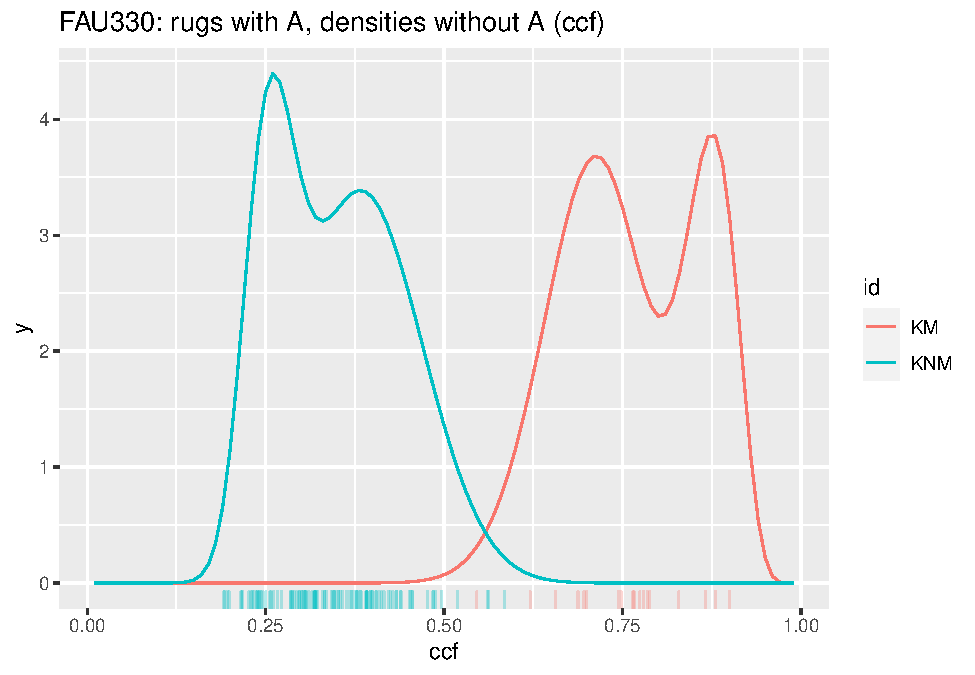
\includegraphics[width=0.7\linewidth]{writeup_files/figure-latex/unnamed-chunk-2-1} 

}

\caption{Densities from training, rugs from test}\label{fig:unnamed-chunk-2}
\end{figure}

\hypertarget{the-following-content-is-help-information-of-the-elsevier-template-keep-for-reference-for-a-while}{%
\section{The following content is help information of the Elsevier
template (keep for reference for a
while)}\label{the-following-content-is-help-information-of-the-elsevier-template-keep-for-reference-for-a-while}}

\hypertarget{the-elsevier-article-class}{%
\section{The Elsevier article class}\label{the-elsevier-article-class}}

\hypertarget{installation}{%
\paragraph{Installation}\label{installation}}

If the document class \emph{elsarticle} is not available on your
computer, you can download and install the system package
\emph{texlive-publishers} (Linux) or install the LaTeX package
\emph{elsarticle} using the package manager of your TeX installation,
which is typically TeX Live or MikTeX.

\hypertarget{usage}{%
\paragraph{Usage}\label{usage}}

Once the package is properly installed, you can use the document class
\emph{elsarticle} to create a manuscript. Please make sure that your
manuscript follows the guidelines in the Guide for Authors of the
relevant journal. It is not necessary to typeset your manuscript in
exactly the same way as an article, unless you are submitting to a
camera-ready copy (CRC) journal.

\hypertarget{functionality}{%
\paragraph{Functionality}\label{functionality}}

The Elsevier article class is based on the standard article class and
supports almost all of the functionality of that class. In addition, it
features commands and options to format the

\begin{itemize}
\item
  document style
\item
  baselineskip
\item
  front matter
\item
  keywords and MSC codes
\item
  theorems, definitions and proofs
\item
  lables of enumerations
\item
  citation style and labeling.
\end{itemize}

\hypertarget{front-matter}{%
\section{Front matter}\label{front-matter}}

The author names and affiliations could be formatted in two ways:

\begin{enumerate}
\def\labelenumi{(\arabic{enumi})}
\item
  Group the authors per affiliation.
\item
  Use footnotes to indicate the affiliations.
\end{enumerate}

See the front matter of this document for examples. You are recommended
to conform your choice to the journal you are submitting to.

\hypertarget{bibliography-styles}{%
\section{Bibliography styles}\label{bibliography-styles}}

There are various bibliography styles available. You can select the
style of your choice in the preamble of this document. These styles are
Elsevier styles based on standard styles like Harvard and Vancouver.
Please use BibTeX to generate your bibliography and include DOIs
whenever available.

\hypertarget{references}{%
\section*{References}\label{references}}
\addcontentsline{toc}{section}{References}

\hypertarget{refs}{}
\leavevmode\hypertarget{ref-Hare2016}{}%
Hare, E., Hofmann, H., Carriquiry, A., 2016. Automatic matching of
bullet land impressions. Annals of Applied Statistics 11, 2332--2356.

\leavevmode\hypertarget{ref-Council2009}{}%
National Research Council, 2009. Strengthening forensic science in the
united states: A path forward, Strengthening Forensic Science in the
United States: A Path Forward. National Academies Press.
doi:\href{https://doi.org/10.17226/12589}{10.17226/12589}


\end{document}


